% Generated from pinned Kolibri results; full precision remains in results.json.
% DescriptiveCI: pointwise 95% paired-block bootstrap, not the primary family bounds.
% Primary bounds: Astra inclusive, two-comparison family 95%, individual 97.5%.
% not run / not planned / not reported / unavailable are not numerical zeros.
\newcommand{\KEXMainAstraExplicitHHMissing}{0}
\newcommand{\KEXMainAstraExplicitHHNegative}{32}
\newcommand{\KEXMainAstraExplicitHHObserved}{32}
\newcommand{\KEXMainAstraExplicitHHPlanned}{32}
\newcommand{\KEXMainAstraExplicitHHPositive}{0}
\newcommand{\KEXMainAstraExplicitHSMissing}{0}
\newcommand{\KEXMainAstraExplicitHSNegative}{32}
\newcommand{\KEXMainAstraExplicitHSObserved}{32}
\newcommand{\KEXMainAstraExplicitHSPlanned}{32}
\newcommand{\KEXMainAstraExplicitHSPositive}{0}
\newcommand{\KEXMainAstraExplicitHShamMissing}{0}
\newcommand{\KEXMainAstraExplicitHShamNegative}{32}
\newcommand{\KEXMainAstraExplicitHShamObserved}{32}
\newcommand{\KEXMainAstraExplicitHShamPlanned}{32}
\newcommand{\KEXMainAstraExplicitHShamPositive}{0}
\newcommand{\KEXMainAstraExplicitMissing}{0}
\newcommand{\KEXMainAstraExplicitNHMissing}{0}
\newcommand{\KEXMainAstraExplicitNHNegative}{32}
\newcommand{\KEXMainAstraExplicitNHObserved}{32}
\newcommand{\KEXMainAstraExplicitNHPlanned}{32}
\newcommand{\KEXMainAstraExplicitNHPositive}{0}
\newcommand{\KEXMainAstraExplicitNSMissing}{0}
\newcommand{\KEXMainAstraExplicitNSNHCompleteBlocks}{32}
\newcommand{\KEXMainAstraExplicitNSNHCompleteEstimate}{0.00}
\newcommand{\KEXMainAstraExplicitNSNHDescriptiveCI}{[0.00, 0.00]}
\newcommand{\KEXMainAstraExplicitNSNHMissingBlocks}{0}
\newcommand{\KEXMainAstraExplicitNSNHMissingLabelBounds}{[0.00, 0.00]}
\newcommand{\KEXMainAstraExplicitNSNHPlannedBlocks}{32}
\newcommand{\KEXMainAstraExplicitNSNegative}{32}
\newcommand{\KEXMainAstraExplicitNSObserved}{32}
\newcommand{\KEXMainAstraExplicitNSPlanned}{32}
\newcommand{\KEXMainAstraExplicitNSPositive}{0}
\newcommand{\KEXMainAstraExplicitNegative}{209}
\newcommand{\KEXMainAstraExplicitObserved}{256}
\newcommand{\KEXMainAstraExplicitPlanned}{256}
\newcommand{\KEXMainAstraExplicitPositive}{47}
\newcommand{\KEXMainAstraExplicitSHHSCompleteBlocks}{32}
\newcommand{\KEXMainAstraExplicitSHHSCompleteEstimate}{0.38}
\newcommand{\KEXMainAstraExplicitSHHSDescriptiveCI}{[0.25, 0.50]}
\newcommand{\KEXMainAstraExplicitSHHSMissingBlocks}{0}
\newcommand{\KEXMainAstraExplicitSHHSMissingLabelBounds}{[0.38, 0.38]}
\newcommand{\KEXMainAstraExplicitSHHSPlannedBlocks}{32}
\newcommand{\KEXMainAstraExplicitSHMissing}{0}
\newcommand{\KEXMainAstraExplicitSHNegative}{20}
\newcommand{\KEXMainAstraExplicitSHObserved}{32}
\newcommand{\KEXMainAstraExplicitSHPlanned}{32}
\newcommand{\KEXMainAstraExplicitSHPositive}{12}
\newcommand{\KEXMainAstraExplicitSSMissing}{0}
\newcommand{\KEXMainAstraExplicitSSNegative}{16}
\newcommand{\KEXMainAstraExplicitSSObserved}{32}
\newcommand{\KEXMainAstraExplicitSSPlanned}{32}
\newcommand{\KEXMainAstraExplicitSSPositive}{16}
\newcommand{\KEXMainAstraExplicitSShamMissing}{0}
\newcommand{\KEXMainAstraExplicitSShamNegative}{13}
\newcommand{\KEXMainAstraExplicitSShamObserved}{32}
\newcommand{\KEXMainAstraExplicitSShamPlanned}{32}
\newcommand{\KEXMainAstraExplicitSShamPositive}{19}
\newcommand{\KEXMainAstraInclusiveHHMissing}{0}
\newcommand{\KEXMainAstraInclusiveHHNegative}{32}
\newcommand{\KEXMainAstraInclusiveHHObserved}{32}
\newcommand{\KEXMainAstraInclusiveHHPlanned}{32}
\newcommand{\KEXMainAstraInclusiveHHPositive}{0}
\newcommand{\KEXMainAstraInclusiveHSMissing}{0}
\newcommand{\KEXMainAstraInclusiveHSNegative}{32}
\newcommand{\KEXMainAstraInclusiveHSObserved}{32}
\newcommand{\KEXMainAstraInclusiveHSPlanned}{32}
\newcommand{\KEXMainAstraInclusiveHSPositive}{0}
\newcommand{\KEXMainAstraInclusiveHShamMissing}{0}
\newcommand{\KEXMainAstraInclusiveHShamNegative}{32}
\newcommand{\KEXMainAstraInclusiveHShamObserved}{32}
\newcommand{\KEXMainAstraInclusiveHShamPlanned}{32}
\newcommand{\KEXMainAstraInclusiveHShamPositive}{0}
\newcommand{\KEXMainAstraInclusiveMissing}{0}
\newcommand{\KEXMainAstraInclusiveNHMissing}{0}
\newcommand{\KEXMainAstraInclusiveNHNegative}{32}
\newcommand{\KEXMainAstraInclusiveNHObserved}{32}
\newcommand{\KEXMainAstraInclusiveNHPlanned}{32}
\newcommand{\KEXMainAstraInclusiveNHPositive}{0}
\newcommand{\KEXMainAstraInclusiveNSMissing}{0}
\newcommand{\KEXMainAstraInclusiveNSNHCompleteBlocks}{32}
\newcommand{\KEXMainAstraInclusiveNSNHCompleteEstimate}{0.00}
\newcommand{\KEXMainAstraInclusiveNSNHDescriptiveCI}{[0.00, 0.00]}
\newcommand{\KEXMainAstraInclusiveNSNHMissingBlocks}{0}
\newcommand{\KEXMainAstraInclusiveNSNHMissingLabelBounds}{[0.00, 0.00]}
\newcommand{\KEXMainAstraInclusiveNSNHPlannedBlocks}{32}
\newcommand{\KEXMainAstraInclusiveNSNegative}{32}
\newcommand{\KEXMainAstraInclusiveNSObserved}{32}
\newcommand{\KEXMainAstraInclusiveNSPlanned}{32}
\newcommand{\KEXMainAstraInclusiveNSPositive}{0}
\newcommand{\KEXMainAstraInclusiveNegative}{197}
\newcommand{\KEXMainAstraInclusiveObserved}{256}
\newcommand{\KEXMainAstraInclusivePlanned}{256}
\newcommand{\KEXMainAstraInclusivePositive}{59}
\newcommand{\KEXMainAstraInclusiveSHHSCompleteBlocks}{32}
\newcommand{\KEXMainAstraInclusiveSHHSCompleteEstimate}{0.50}
\newcommand{\KEXMainAstraInclusiveSHHSDescriptiveCI}{[0.34, 0.66]}
\newcommand{\KEXMainAstraInclusiveSHHSMissingBlocks}{0}
\newcommand{\KEXMainAstraInclusiveSHHSMissingLabelBounds}{[0.50, 0.50]}
\newcommand{\KEXMainAstraInclusiveSHHSPlannedBlocks}{32}
\newcommand{\KEXMainAstraInclusiveSHMissing}{0}
\newcommand{\KEXMainAstraInclusiveSHNegative}{16}
\newcommand{\KEXMainAstraInclusiveSHObserved}{32}
\newcommand{\KEXMainAstraInclusiveSHPlanned}{32}
\newcommand{\KEXMainAstraInclusiveSHPositive}{16}
\newcommand{\KEXMainAstraInclusiveSSMissing}{0}
\newcommand{\KEXMainAstraInclusiveSSNegative}{12}
\newcommand{\KEXMainAstraInclusiveSSObserved}{32}
\newcommand{\KEXMainAstraInclusiveSSPlanned}{32}
\newcommand{\KEXMainAstraInclusiveSSPositive}{20}
\newcommand{\KEXMainAstraInclusiveSShamMissing}{0}
\newcommand{\KEXMainAstraInclusiveSShamNegative}{9}
\newcommand{\KEXMainAstraInclusiveSShamObserved}{32}
\newcommand{\KEXMainAstraInclusiveSShamPlanned}{32}
\newcommand{\KEXMainAstraInclusiveSShamPositive}{23}
\newcommand{\KEXMainAstraPaperHHMissing}{0}
\newcommand{\KEXMainAstraPaperHHNegative}{32}
\newcommand{\KEXMainAstraPaperHHObserved}{32}
\newcommand{\KEXMainAstraPaperHHPlanned}{32}
\newcommand{\KEXMainAstraPaperHHPositive}{0}
\newcommand{\KEXMainAstraPaperHSMissing}{0}
\newcommand{\KEXMainAstraPaperHSNegative}{32}
\newcommand{\KEXMainAstraPaperHSObserved}{32}
\newcommand{\KEXMainAstraPaperHSPlanned}{32}
\newcommand{\KEXMainAstraPaperHSPositive}{0}
\newcommand{\KEXMainAstraPaperHShamMissing}{0}
\newcommand{\KEXMainAstraPaperHShamNegative}{32}
\newcommand{\KEXMainAstraPaperHShamObserved}{32}
\newcommand{\KEXMainAstraPaperHShamPlanned}{32}
\newcommand{\KEXMainAstraPaperHShamPositive}{0}
\newcommand{\KEXMainAstraPaperMissing}{0}
\newcommand{\KEXMainAstraPaperNHMissing}{0}
\newcommand{\KEXMainAstraPaperNHNegative}{32}
\newcommand{\KEXMainAstraPaperNHObserved}{32}
\newcommand{\KEXMainAstraPaperNHPlanned}{32}
\newcommand{\KEXMainAstraPaperNHPositive}{0}
\newcommand{\KEXMainAstraPaperNSMissing}{0}
\newcommand{\KEXMainAstraPaperNSNHCompleteBlocks}{32}
\newcommand{\KEXMainAstraPaperNSNHCompleteEstimate}{0.00}
\newcommand{\KEXMainAstraPaperNSNHDescriptiveCI}{[0.00, 0.00]}
\newcommand{\KEXMainAstraPaperNSNHMissingBlocks}{0}
\newcommand{\KEXMainAstraPaperNSNHMissingLabelBounds}{[0.00, 0.00]}
\newcommand{\KEXMainAstraPaperNSNHPlannedBlocks}{32}
\newcommand{\KEXMainAstraPaperNSNegative}{32}
\newcommand{\KEXMainAstraPaperNSObserved}{32}
\newcommand{\KEXMainAstraPaperNSPlanned}{32}
\newcommand{\KEXMainAstraPaperNSPositive}{0}
\newcommand{\KEXMainAstraPaperNegative}{181}
\newcommand{\KEXMainAstraPaperObserved}{256}
\newcommand{\KEXMainAstraPaperPlanned}{256}
\newcommand{\KEXMainAstraPaperPositive}{75}
\newcommand{\KEXMainAstraPaperSHHSCompleteBlocks}{32}
\newcommand{\KEXMainAstraPaperSHHSCompleteEstimate}{0.69}
\newcommand{\KEXMainAstraPaperSHHSDescriptiveCI}{[0.53, 0.84]}
\newcommand{\KEXMainAstraPaperSHHSMissingBlocks}{0}
\newcommand{\KEXMainAstraPaperSHHSMissingLabelBounds}{[0.69, 0.69]}
\newcommand{\KEXMainAstraPaperSHHSPlannedBlocks}{32}
\newcommand{\KEXMainAstraPaperSHMissing}{0}
\newcommand{\KEXMainAstraPaperSHNegative}{10}
\newcommand{\KEXMainAstraPaperSHObserved}{32}
\newcommand{\KEXMainAstraPaperSHPlanned}{32}
\newcommand{\KEXMainAstraPaperSHPositive}{22}
\newcommand{\KEXMainAstraPaperSSMissing}{0}
\newcommand{\KEXMainAstraPaperSSNegative}{6}
\newcommand{\KEXMainAstraPaperSSObserved}{32}
\newcommand{\KEXMainAstraPaperSSPlanned}{32}
\newcommand{\KEXMainAstraPaperSSPositive}{26}
\newcommand{\KEXMainAstraPaperSShamMissing}{0}
\newcommand{\KEXMainAstraPaperSShamNegative}{5}
\newcommand{\KEXMainAstraPaperSShamObserved}{32}
\newcommand{\KEXMainAstraPaperSShamPlanned}{32}
\newcommand{\KEXMainAstraPaperSShamPositive}{27}
\newcommand{\KEXMainMissingFinalContent}{0}
\newcommand{\KEXMainOpusExplicitHHMissing}{0}
\newcommand{\KEXMainOpusExplicitHHNegative}{32}
\newcommand{\KEXMainOpusExplicitHHObserved}{32}
\newcommand{\KEXMainOpusExplicitHHPlanned}{32}
\newcommand{\KEXMainOpusExplicitHHPositive}{0}
\newcommand{\KEXMainOpusExplicitHSMissing}{0}
\newcommand{\KEXMainOpusExplicitHSNegative}{32}
\newcommand{\KEXMainOpusExplicitHSObserved}{32}
\newcommand{\KEXMainOpusExplicitHSPlanned}{32}
\newcommand{\KEXMainOpusExplicitHSPositive}{0}
\newcommand{\KEXMainOpusExplicitHShamMissing}{0}
\newcommand{\KEXMainOpusExplicitHShamNegative}{32}
\newcommand{\KEXMainOpusExplicitHShamObserved}{32}
\newcommand{\KEXMainOpusExplicitHShamPlanned}{32}
\newcommand{\KEXMainOpusExplicitHShamPositive}{0}
\newcommand{\KEXMainOpusExplicitMissing}{0}
\newcommand{\KEXMainOpusExplicitNHMissing}{0}
\newcommand{\KEXMainOpusExplicitNHNegative}{32}
\newcommand{\KEXMainOpusExplicitNHObserved}{32}
\newcommand{\KEXMainOpusExplicitNHPlanned}{32}
\newcommand{\KEXMainOpusExplicitNHPositive}{0}
\newcommand{\KEXMainOpusExplicitNSMissing}{0}
\newcommand{\KEXMainOpusExplicitNSNHCompleteBlocks}{32}
\newcommand{\KEXMainOpusExplicitNSNHCompleteEstimate}{0.00}
\newcommand{\KEXMainOpusExplicitNSNHDescriptiveCI}{[0.00, 0.00]}
\newcommand{\KEXMainOpusExplicitNSNHMissingBlocks}{0}
\newcommand{\KEXMainOpusExplicitNSNHMissingLabelBounds}{[0.00, 0.00]}
\newcommand{\KEXMainOpusExplicitNSNHPlannedBlocks}{32}
\newcommand{\KEXMainOpusExplicitNSNegative}{32}
\newcommand{\KEXMainOpusExplicitNSObserved}{32}
\newcommand{\KEXMainOpusExplicitNSPlanned}{32}
\newcommand{\KEXMainOpusExplicitNSPositive}{0}
\newcommand{\KEXMainOpusExplicitNegative}{205}
\newcommand{\KEXMainOpusExplicitObserved}{256}
\newcommand{\KEXMainOpusExplicitPlanned}{256}
\newcommand{\KEXMainOpusExplicitPositive}{51}
\newcommand{\KEXMainOpusExplicitSHHSCompleteBlocks}{32}
\newcommand{\KEXMainOpusExplicitSHHSCompleteEstimate}{0.38}
\newcommand{\KEXMainOpusExplicitSHHSDescriptiveCI}{[0.25, 0.50]}
\newcommand{\KEXMainOpusExplicitSHHSMissingBlocks}{0}
\newcommand{\KEXMainOpusExplicitSHHSMissingLabelBounds}{[0.38, 0.38]}
\newcommand{\KEXMainOpusExplicitSHHSPlannedBlocks}{32}
\newcommand{\KEXMainOpusExplicitSHMissing}{0}
\newcommand{\KEXMainOpusExplicitSHNegative}{20}
\newcommand{\KEXMainOpusExplicitSHObserved}{32}
\newcommand{\KEXMainOpusExplicitSHPlanned}{32}
\newcommand{\KEXMainOpusExplicitSHPositive}{12}
\newcommand{\KEXMainOpusExplicitSSMissing}{0}
\newcommand{\KEXMainOpusExplicitSSNegative}{12}
\newcommand{\KEXMainOpusExplicitSSObserved}{32}
\newcommand{\KEXMainOpusExplicitSSPlanned}{32}
\newcommand{\KEXMainOpusExplicitSSPositive}{20}
\newcommand{\KEXMainOpusExplicitSShamMissing}{0}
\newcommand{\KEXMainOpusExplicitSShamNegative}{13}
\newcommand{\KEXMainOpusExplicitSShamObserved}{32}
\newcommand{\KEXMainOpusExplicitSShamPlanned}{32}
\newcommand{\KEXMainOpusExplicitSShamPositive}{19}
\newcommand{\KEXMainOpusInclusiveHHMissing}{0}
\newcommand{\KEXMainOpusInclusiveHHNegative}{32}
\newcommand{\KEXMainOpusInclusiveHHObserved}{32}
\newcommand{\KEXMainOpusInclusiveHHPlanned}{32}
\newcommand{\KEXMainOpusInclusiveHHPositive}{0}
\newcommand{\KEXMainOpusInclusiveHSMissing}{0}
\newcommand{\KEXMainOpusInclusiveHSNegative}{32}
\newcommand{\KEXMainOpusInclusiveHSObserved}{32}
\newcommand{\KEXMainOpusInclusiveHSPlanned}{32}
\newcommand{\KEXMainOpusInclusiveHSPositive}{0}
\newcommand{\KEXMainOpusInclusiveHShamMissing}{0}
\newcommand{\KEXMainOpusInclusiveHShamNegative}{32}
\newcommand{\KEXMainOpusInclusiveHShamObserved}{32}
\newcommand{\KEXMainOpusInclusiveHShamPlanned}{32}
\newcommand{\KEXMainOpusInclusiveHShamPositive}{0}
\newcommand{\KEXMainOpusInclusiveMissing}{0}
\newcommand{\KEXMainOpusInclusiveNHMissing}{0}
\newcommand{\KEXMainOpusInclusiveNHNegative}{32}
\newcommand{\KEXMainOpusInclusiveNHObserved}{32}
\newcommand{\KEXMainOpusInclusiveNHPlanned}{32}
\newcommand{\KEXMainOpusInclusiveNHPositive}{0}
\newcommand{\KEXMainOpusInclusiveNSMissing}{0}
\newcommand{\KEXMainOpusInclusiveNSNHCompleteBlocks}{32}
\newcommand{\KEXMainOpusInclusiveNSNHCompleteEstimate}{0.00}
\newcommand{\KEXMainOpusInclusiveNSNHDescriptiveCI}{[0.00, 0.00]}
\newcommand{\KEXMainOpusInclusiveNSNHMissingBlocks}{0}
\newcommand{\KEXMainOpusInclusiveNSNHMissingLabelBounds}{[0.00, 0.00]}
\newcommand{\KEXMainOpusInclusiveNSNHPlannedBlocks}{32}
\newcommand{\KEXMainOpusInclusiveNSNegative}{32}
\newcommand{\KEXMainOpusInclusiveNSObserved}{32}
\newcommand{\KEXMainOpusInclusiveNSPlanned}{32}
\newcommand{\KEXMainOpusInclusiveNSPositive}{0}
\newcommand{\KEXMainOpusInclusiveNegative}{187}
\newcommand{\KEXMainOpusInclusiveObserved}{256}
\newcommand{\KEXMainOpusInclusivePlanned}{256}
\newcommand{\KEXMainOpusInclusivePositive}{69}
\newcommand{\KEXMainOpusInclusiveSHHSCompleteBlocks}{32}
\newcommand{\KEXMainOpusInclusiveSHHSCompleteEstimate}{0.63}
\newcommand{\KEXMainOpusInclusiveSHHSDescriptiveCI}{[0.47, 0.78]}
\newcommand{\KEXMainOpusInclusiveSHHSMissingBlocks}{0}
\newcommand{\KEXMainOpusInclusiveSHHSMissingLabelBounds}{[0.63, 0.63]}
\newcommand{\KEXMainOpusInclusiveSHHSPlannedBlocks}{32}
\newcommand{\KEXMainOpusInclusiveSHMissing}{0}
\newcommand{\KEXMainOpusInclusiveSHNegative}{12}
\newcommand{\KEXMainOpusInclusiveSHObserved}{32}
\newcommand{\KEXMainOpusInclusiveSHPlanned}{32}
\newcommand{\KEXMainOpusInclusiveSHPositive}{20}
\newcommand{\KEXMainOpusInclusiveSSMissing}{0}
\newcommand{\KEXMainOpusInclusiveSSNegative}{9}
\newcommand{\KEXMainOpusInclusiveSSObserved}{32}
\newcommand{\KEXMainOpusInclusiveSSPlanned}{32}
\newcommand{\KEXMainOpusInclusiveSSPositive}{23}
\newcommand{\KEXMainOpusInclusiveSShamMissing}{0}
\newcommand{\KEXMainOpusInclusiveSShamNegative}{6}
\newcommand{\KEXMainOpusInclusiveSShamObserved}{32}
\newcommand{\KEXMainOpusInclusiveSShamPlanned}{32}
\newcommand{\KEXMainOpusInclusiveSShamPositive}{26}
\newcommand{\KEXMainOpusPaperHHMissing}{0}
\newcommand{\KEXMainOpusPaperHHNegative}{32}
\newcommand{\KEXMainOpusPaperHHObserved}{32}
\newcommand{\KEXMainOpusPaperHHPlanned}{32}
\newcommand{\KEXMainOpusPaperHHPositive}{0}
\newcommand{\KEXMainOpusPaperHSMissing}{0}
\newcommand{\KEXMainOpusPaperHSNegative}{32}
\newcommand{\KEXMainOpusPaperHSObserved}{32}
\newcommand{\KEXMainOpusPaperHSPlanned}{32}
\newcommand{\KEXMainOpusPaperHSPositive}{0}
\newcommand{\KEXMainOpusPaperHShamMissing}{0}
\newcommand{\KEXMainOpusPaperHShamNegative}{32}
\newcommand{\KEXMainOpusPaperHShamObserved}{32}
\newcommand{\KEXMainOpusPaperHShamPlanned}{32}
\newcommand{\KEXMainOpusPaperHShamPositive}{0}
\newcommand{\KEXMainOpusPaperMissing}{0}
\newcommand{\KEXMainOpusPaperNHMissing}{0}
\newcommand{\KEXMainOpusPaperNHNegative}{32}
\newcommand{\KEXMainOpusPaperNHObserved}{32}
\newcommand{\KEXMainOpusPaperNHPlanned}{32}
\newcommand{\KEXMainOpusPaperNHPositive}{0}
\newcommand{\KEXMainOpusPaperNSMissing}{0}
\newcommand{\KEXMainOpusPaperNSNHCompleteBlocks}{32}
\newcommand{\KEXMainOpusPaperNSNHCompleteEstimate}{0.00}
\newcommand{\KEXMainOpusPaperNSNHDescriptiveCI}{[0.00, 0.00]}
\newcommand{\KEXMainOpusPaperNSNHMissingBlocks}{0}
\newcommand{\KEXMainOpusPaperNSNHMissingLabelBounds}{[0.00, 0.00]}
\newcommand{\KEXMainOpusPaperNSNHPlannedBlocks}{32}
\newcommand{\KEXMainOpusPaperNSNegative}{32}
\newcommand{\KEXMainOpusPaperNSObserved}{32}
\newcommand{\KEXMainOpusPaperNSPlanned}{32}
\newcommand{\KEXMainOpusPaperNSPositive}{0}
\newcommand{\KEXMainOpusPaperNegative}{175}
\newcommand{\KEXMainOpusPaperObserved}{256}
\newcommand{\KEXMainOpusPaperPlanned}{256}
\newcommand{\KEXMainOpusPaperPositive}{81}
\newcommand{\KEXMainOpusPaperSHHSCompleteBlocks}{32}
\newcommand{\KEXMainOpusPaperSHHSCompleteEstimate}{0.75}
\newcommand{\KEXMainOpusPaperSHHSDescriptiveCI}{[0.63, 0.88]}
\newcommand{\KEXMainOpusPaperSHHSMissingBlocks}{0}
\newcommand{\KEXMainOpusPaperSHHSMissingLabelBounds}{[0.75, 0.75]}
\newcommand{\KEXMainOpusPaperSHHSPlannedBlocks}{32}
\newcommand{\KEXMainOpusPaperSHMissing}{0}
\newcommand{\KEXMainOpusPaperSHNegative}{8}
\newcommand{\KEXMainOpusPaperSHObserved}{32}
\newcommand{\KEXMainOpusPaperSHPlanned}{32}
\newcommand{\KEXMainOpusPaperSHPositive}{24}
\newcommand{\KEXMainOpusPaperSSMissing}{0}
\newcommand{\KEXMainOpusPaperSSNegative}{4}
\newcommand{\KEXMainOpusPaperSSObserved}{32}
\newcommand{\KEXMainOpusPaperSSPlanned}{32}
\newcommand{\KEXMainOpusPaperSSPositive}{28}
\newcommand{\KEXMainOpusPaperSShamMissing}{0}
\newcommand{\KEXMainOpusPaperSShamNegative}{3}
\newcommand{\KEXMainOpusPaperSShamObserved}{32}
\newcommand{\KEXMainOpusPaperSShamPlanned}{32}
\newcommand{\KEXMainOpusPaperSShamPositive}{29}
\newcommand{\KEXMainPlannedFinals}{256}
\newcommand{\KEXMainState}{collected}
\newcommand{\KEXPrimaryAstraInclusiveNSNHBounds}{[-0.52, 0.52]}
\newcommand{\KEXPrimaryAstraInclusiveNSNHCompleteBlocks}{32}
\newcommand{\KEXPrimaryAstraInclusiveNSNHMissingBlocks}{0}
\newcommand{\KEXPrimaryAstraInclusiveNSNHPlannedBlocks}{32}
\newcommand{\KEXPrimaryAstraInclusiveSHHSBounds}{[-0.02, 1.00]}
\newcommand{\KEXPrimaryAstraInclusiveSHHSCompleteBlocks}{32}
\newcommand{\KEXPrimaryAstraInclusiveSHHSMissingBlocks}{0}
\newcommand{\KEXPrimaryAstraInclusiveSHHSPlannedBlocks}{32}
\newcommand{\KEXPrimaryFamilySize}{2}
\newcommand{\KEXPrimaryFamilywiseConfidence}{95.00\%}
\newcommand{\KEXPrimaryIndividualConfidence}{97.50\%}
\newcommand{\KEXPrimaryMethod}{Bonferroni bounded Hoeffding}
\newcommand{\KEXQualification}{passed}
\newcommand{\KEXScreenAstraExplicitHHMissing}{0}
\newcommand{\KEXScreenAstraExplicitHHNegative}{12}
\newcommand{\KEXScreenAstraExplicitHHObserved}{12}
\newcommand{\KEXScreenAstraExplicitHHPlanned}{12}
\newcommand{\KEXScreenAstraExplicitHHPositive}{0}
\newcommand{\KEXScreenAstraExplicitHSMissing}{0}
\newcommand{\KEXScreenAstraExplicitHSNegative}{12}
\newcommand{\KEXScreenAstraExplicitHSObserved}{12}
\newcommand{\KEXScreenAstraExplicitHSPlanned}{12}
\newcommand{\KEXScreenAstraExplicitHSPositive}{0}
\newcommand{\KEXScreenAstraExplicitHShamMissing}{not planned}
\newcommand{\KEXScreenAstraExplicitHShamNegative}{not planned}
\newcommand{\KEXScreenAstraExplicitHShamObserved}{not planned}
\newcommand{\KEXScreenAstraExplicitHShamPlanned}{not planned}
\newcommand{\KEXScreenAstraExplicitHShamPositive}{not planned}
\newcommand{\KEXScreenAstraExplicitMissing}{1}
\newcommand{\KEXScreenAstraExplicitNHMissing}{not planned}
\newcommand{\KEXScreenAstraExplicitNHNegative}{not planned}
\newcommand{\KEXScreenAstraExplicitNHObserved}{not planned}
\newcommand{\KEXScreenAstraExplicitNHPlanned}{not planned}
\newcommand{\KEXScreenAstraExplicitNHPositive}{not planned}
\newcommand{\KEXScreenAstraExplicitNSMissing}{not planned}
\newcommand{\KEXScreenAstraExplicitNSNHCompleteBlocks}{not planned}
\newcommand{\KEXScreenAstraExplicitNSNHCompleteEstimate}{not planned}
\newcommand{\KEXScreenAstraExplicitNSNHDescriptiveCI}{not planned}
\newcommand{\KEXScreenAstraExplicitNSNHMissingBlocks}{not planned}
\newcommand{\KEXScreenAstraExplicitNSNHMissingLabelBounds}{not planned}
\newcommand{\KEXScreenAstraExplicitNSNHPlannedBlocks}{not planned}
\newcommand{\KEXScreenAstraExplicitNSNegative}{not planned}
\newcommand{\KEXScreenAstraExplicitNSObserved}{not planned}
\newcommand{\KEXScreenAstraExplicitNSPlanned}{not planned}
\newcommand{\KEXScreenAstraExplicitNSPositive}{not planned}
\newcommand{\KEXScreenAstraExplicitNegative}{41}
\newcommand{\KEXScreenAstraExplicitObserved}{47}
\newcommand{\KEXScreenAstraExplicitPlanned}{48}
\newcommand{\KEXScreenAstraExplicitPositive}{6}
\newcommand{\KEXScreenAstraExplicitSHHSCompleteBlocks}{12}
\newcommand{\KEXScreenAstraExplicitSHHSCompleteEstimate}{0.17}
\newcommand{\KEXScreenAstraExplicitSHHSDescriptiveCI}{[0.00, 0.33]}
\newcommand{\KEXScreenAstraExplicitSHHSMissingBlocks}{0}
\newcommand{\KEXScreenAstraExplicitSHHSMissingLabelBounds}{[0.17, 0.17]}
\newcommand{\KEXScreenAstraExplicitSHHSPlannedBlocks}{12}
\newcommand{\KEXScreenAstraExplicitSHMissing}{0}
\newcommand{\KEXScreenAstraExplicitSHNegative}{10}
\newcommand{\KEXScreenAstraExplicitSHObserved}{12}
\newcommand{\KEXScreenAstraExplicitSHPlanned}{12}
\newcommand{\KEXScreenAstraExplicitSHPositive}{2}
\newcommand{\KEXScreenAstraExplicitSSMissing}{1}
\newcommand{\KEXScreenAstraExplicitSSNegative}{7}
\newcommand{\KEXScreenAstraExplicitSSObserved}{11}
\newcommand{\KEXScreenAstraExplicitSSPlanned}{12}
\newcommand{\KEXScreenAstraExplicitSSPositive}{4}
\newcommand{\KEXScreenAstraExplicitSShamMissing}{not planned}
\newcommand{\KEXScreenAstraExplicitSShamNegative}{not planned}
\newcommand{\KEXScreenAstraExplicitSShamObserved}{not planned}
\newcommand{\KEXScreenAstraExplicitSShamPlanned}{not planned}
\newcommand{\KEXScreenAstraExplicitSShamPositive}{not planned}
\newcommand{\KEXScreenAstraInclusiveHHMissing}{0}
\newcommand{\KEXScreenAstraInclusiveHHNegative}{12}
\newcommand{\KEXScreenAstraInclusiveHHObserved}{12}
\newcommand{\KEXScreenAstraInclusiveHHPlanned}{12}
\newcommand{\KEXScreenAstraInclusiveHHPositive}{0}
\newcommand{\KEXScreenAstraInclusiveHSMissing}{0}
\newcommand{\KEXScreenAstraInclusiveHSNegative}{12}
\newcommand{\KEXScreenAstraInclusiveHSObserved}{12}
\newcommand{\KEXScreenAstraInclusiveHSPlanned}{12}
\newcommand{\KEXScreenAstraInclusiveHSPositive}{0}
\newcommand{\KEXScreenAstraInclusiveHShamMissing}{not planned}
\newcommand{\KEXScreenAstraInclusiveHShamNegative}{not planned}
\newcommand{\KEXScreenAstraInclusiveHShamObserved}{not planned}
\newcommand{\KEXScreenAstraInclusiveHShamPlanned}{not planned}
\newcommand{\KEXScreenAstraInclusiveHShamPositive}{not planned}
\newcommand{\KEXScreenAstraInclusiveMissing}{1}
\newcommand{\KEXScreenAstraInclusiveNHMissing}{not planned}
\newcommand{\KEXScreenAstraInclusiveNHNegative}{not planned}
\newcommand{\KEXScreenAstraInclusiveNHObserved}{not planned}
\newcommand{\KEXScreenAstraInclusiveNHPlanned}{not planned}
\newcommand{\KEXScreenAstraInclusiveNHPositive}{not planned}
\newcommand{\KEXScreenAstraInclusiveNSMissing}{not planned}
\newcommand{\KEXScreenAstraInclusiveNSNHCompleteBlocks}{not planned}
\newcommand{\KEXScreenAstraInclusiveNSNHCompleteEstimate}{not planned}
\newcommand{\KEXScreenAstraInclusiveNSNHDescriptiveCI}{not planned}
\newcommand{\KEXScreenAstraInclusiveNSNHMissingBlocks}{not planned}
\newcommand{\KEXScreenAstraInclusiveNSNHMissingLabelBounds}{not planned}
\newcommand{\KEXScreenAstraInclusiveNSNHPlannedBlocks}{not planned}
\newcommand{\KEXScreenAstraInclusiveNSNegative}{not planned}
\newcommand{\KEXScreenAstraInclusiveNSObserved}{not planned}
\newcommand{\KEXScreenAstraInclusiveNSPlanned}{not planned}
\newcommand{\KEXScreenAstraInclusiveNSPositive}{not planned}
\newcommand{\KEXScreenAstraInclusiveNegative}{38}
\newcommand{\KEXScreenAstraInclusiveObserved}{47}
\newcommand{\KEXScreenAstraInclusivePlanned}{48}
\newcommand{\KEXScreenAstraInclusivePositive}{9}
\newcommand{\KEXScreenAstraInclusiveSHHSCompleteBlocks}{12}
\newcommand{\KEXScreenAstraInclusiveSHHSCompleteEstimate}{0.33}
\newcommand{\KEXScreenAstraInclusiveSHHSDescriptiveCI}{[0.08, 0.58]}
\newcommand{\KEXScreenAstraInclusiveSHHSMissingBlocks}{0}
\newcommand{\KEXScreenAstraInclusiveSHHSMissingLabelBounds}{[0.33, 0.33]}
\newcommand{\KEXScreenAstraInclusiveSHHSPlannedBlocks}{12}
\newcommand{\KEXScreenAstraInclusiveSHMissing}{0}
\newcommand{\KEXScreenAstraInclusiveSHNegative}{8}
\newcommand{\KEXScreenAstraInclusiveSHObserved}{12}
\newcommand{\KEXScreenAstraInclusiveSHPlanned}{12}
\newcommand{\KEXScreenAstraInclusiveSHPositive}{4}
\newcommand{\KEXScreenAstraInclusiveSSMissing}{1}
\newcommand{\KEXScreenAstraInclusiveSSNegative}{6}
\newcommand{\KEXScreenAstraInclusiveSSObserved}{11}
\newcommand{\KEXScreenAstraInclusiveSSPlanned}{12}
\newcommand{\KEXScreenAstraInclusiveSSPositive}{5}
\newcommand{\KEXScreenAstraInclusiveSShamMissing}{not planned}
\newcommand{\KEXScreenAstraInclusiveSShamNegative}{not planned}
\newcommand{\KEXScreenAstraInclusiveSShamObserved}{not planned}
\newcommand{\KEXScreenAstraInclusiveSShamPlanned}{not planned}
\newcommand{\KEXScreenAstraInclusiveSShamPositive}{not planned}
\newcommand{\KEXScreenAstraPaperHHMissing}{0}
\newcommand{\KEXScreenAstraPaperHHNegative}{12}
\newcommand{\KEXScreenAstraPaperHHObserved}{12}
\newcommand{\KEXScreenAstraPaperHHPlanned}{12}
\newcommand{\KEXScreenAstraPaperHHPositive}{0}
\newcommand{\KEXScreenAstraPaperHSMissing}{0}
\newcommand{\KEXScreenAstraPaperHSNegative}{12}
\newcommand{\KEXScreenAstraPaperHSObserved}{12}
\newcommand{\KEXScreenAstraPaperHSPlanned}{12}
\newcommand{\KEXScreenAstraPaperHSPositive}{0}
\newcommand{\KEXScreenAstraPaperHShamMissing}{not planned}
\newcommand{\KEXScreenAstraPaperHShamNegative}{not planned}
\newcommand{\KEXScreenAstraPaperHShamObserved}{not planned}
\newcommand{\KEXScreenAstraPaperHShamPlanned}{not planned}
\newcommand{\KEXScreenAstraPaperHShamPositive}{not planned}
\newcommand{\KEXScreenAstraPaperMissing}{1}
\newcommand{\KEXScreenAstraPaperNHMissing}{not planned}
\newcommand{\KEXScreenAstraPaperNHNegative}{not planned}
\newcommand{\KEXScreenAstraPaperNHObserved}{not planned}
\newcommand{\KEXScreenAstraPaperNHPlanned}{not planned}
\newcommand{\KEXScreenAstraPaperNHPositive}{not planned}
\newcommand{\KEXScreenAstraPaperNSMissing}{not planned}
\newcommand{\KEXScreenAstraPaperNSNHCompleteBlocks}{not planned}
\newcommand{\KEXScreenAstraPaperNSNHCompleteEstimate}{not planned}
\newcommand{\KEXScreenAstraPaperNSNHDescriptiveCI}{not planned}
\newcommand{\KEXScreenAstraPaperNSNHMissingBlocks}{not planned}
\newcommand{\KEXScreenAstraPaperNSNHMissingLabelBounds}{not planned}
\newcommand{\KEXScreenAstraPaperNSNHPlannedBlocks}{not planned}
\newcommand{\KEXScreenAstraPaperNSNegative}{not planned}
\newcommand{\KEXScreenAstraPaperNSObserved}{not planned}
\newcommand{\KEXScreenAstraPaperNSPlanned}{not planned}
\newcommand{\KEXScreenAstraPaperNSPositive}{not planned}
\newcommand{\KEXScreenAstraPaperNegative}{32}
\newcommand{\KEXScreenAstraPaperObserved}{47}
\newcommand{\KEXScreenAstraPaperPlanned}{48}
\newcommand{\KEXScreenAstraPaperPositive}{15}
\newcommand{\KEXScreenAstraPaperSHHSCompleteBlocks}{12}
\newcommand{\KEXScreenAstraPaperSHHSCompleteEstimate}{0.67}
\newcommand{\KEXScreenAstraPaperSHHSDescriptiveCI}{[0.50, 0.83]}
\newcommand{\KEXScreenAstraPaperSHHSMissingBlocks}{0}
\newcommand{\KEXScreenAstraPaperSHHSMissingLabelBounds}{[0.67, 0.67]}
\newcommand{\KEXScreenAstraPaperSHHSPlannedBlocks}{12}
\newcommand{\KEXScreenAstraPaperSHMissing}{0}
\newcommand{\KEXScreenAstraPaperSHNegative}{4}
\newcommand{\KEXScreenAstraPaperSHObserved}{12}
\newcommand{\KEXScreenAstraPaperSHPlanned}{12}
\newcommand{\KEXScreenAstraPaperSHPositive}{8}
\newcommand{\KEXScreenAstraPaperSSMissing}{1}
\newcommand{\KEXScreenAstraPaperSSNegative}{4}
\newcommand{\KEXScreenAstraPaperSSObserved}{11}
\newcommand{\KEXScreenAstraPaperSSPlanned}{12}
\newcommand{\KEXScreenAstraPaperSSPositive}{7}
\newcommand{\KEXScreenAstraPaperSShamMissing}{not planned}
\newcommand{\KEXScreenAstraPaperSShamNegative}{not planned}
\newcommand{\KEXScreenAstraPaperSShamObserved}{not planned}
\newcommand{\KEXScreenAstraPaperSShamPlanned}{not planned}
\newcommand{\KEXScreenAstraPaperSShamPositive}{not planned}
\newcommand{\KEXScreenMissingFinalContent}{1}
\newcommand{\KEXScreenOpusExplicitHHMissing}{0}
\newcommand{\KEXScreenOpusExplicitHHNegative}{12}
\newcommand{\KEXScreenOpusExplicitHHObserved}{12}
\newcommand{\KEXScreenOpusExplicitHHPlanned}{12}
\newcommand{\KEXScreenOpusExplicitHHPositive}{0}
\newcommand{\KEXScreenOpusExplicitHSMissing}{0}
\newcommand{\KEXScreenOpusExplicitHSNegative}{12}
\newcommand{\KEXScreenOpusExplicitHSObserved}{12}
\newcommand{\KEXScreenOpusExplicitHSPlanned}{12}
\newcommand{\KEXScreenOpusExplicitHSPositive}{0}
\newcommand{\KEXScreenOpusExplicitHShamMissing}{not planned}
\newcommand{\KEXScreenOpusExplicitHShamNegative}{not planned}
\newcommand{\KEXScreenOpusExplicitHShamObserved}{not planned}
\newcommand{\KEXScreenOpusExplicitHShamPlanned}{not planned}
\newcommand{\KEXScreenOpusExplicitHShamPositive}{not planned}
\newcommand{\KEXScreenOpusExplicitMissing}{1}
\newcommand{\KEXScreenOpusExplicitNHMissing}{not planned}
\newcommand{\KEXScreenOpusExplicitNHNegative}{not planned}
\newcommand{\KEXScreenOpusExplicitNHObserved}{not planned}
\newcommand{\KEXScreenOpusExplicitNHPlanned}{not planned}
\newcommand{\KEXScreenOpusExplicitNHPositive}{not planned}
\newcommand{\KEXScreenOpusExplicitNSMissing}{not planned}
\newcommand{\KEXScreenOpusExplicitNSNHCompleteBlocks}{not planned}
\newcommand{\KEXScreenOpusExplicitNSNHCompleteEstimate}{not planned}
\newcommand{\KEXScreenOpusExplicitNSNHDescriptiveCI}{not planned}
\newcommand{\KEXScreenOpusExplicitNSNHMissingBlocks}{not planned}
\newcommand{\KEXScreenOpusExplicitNSNHMissingLabelBounds}{not planned}
\newcommand{\KEXScreenOpusExplicitNSNHPlannedBlocks}{not planned}
\newcommand{\KEXScreenOpusExplicitNSNegative}{not planned}
\newcommand{\KEXScreenOpusExplicitNSObserved}{not planned}
\newcommand{\KEXScreenOpusExplicitNSPlanned}{not planned}
\newcommand{\KEXScreenOpusExplicitNSPositive}{not planned}
\newcommand{\KEXScreenOpusExplicitNegative}{38}
\newcommand{\KEXScreenOpusExplicitObserved}{47}
\newcommand{\KEXScreenOpusExplicitPlanned}{48}
\newcommand{\KEXScreenOpusExplicitPositive}{9}
\newcommand{\KEXScreenOpusExplicitSHHSCompleteBlocks}{12}
\newcommand{\KEXScreenOpusExplicitSHHSCompleteEstimate}{0.33}
\newcommand{\KEXScreenOpusExplicitSHHSDescriptiveCI}{[0.17, 0.50]}
\newcommand{\KEXScreenOpusExplicitSHHSMissingBlocks}{0}
\newcommand{\KEXScreenOpusExplicitSHHSMissingLabelBounds}{[0.33, 0.33]}
\newcommand{\KEXScreenOpusExplicitSHHSPlannedBlocks}{12}
\newcommand{\KEXScreenOpusExplicitSHMissing}{0}
\newcommand{\KEXScreenOpusExplicitSHNegative}{8}
\newcommand{\KEXScreenOpusExplicitSHObserved}{12}
\newcommand{\KEXScreenOpusExplicitSHPlanned}{12}
\newcommand{\KEXScreenOpusExplicitSHPositive}{4}
\newcommand{\KEXScreenOpusExplicitSSMissing}{1}
\newcommand{\KEXScreenOpusExplicitSSNegative}{6}
\newcommand{\KEXScreenOpusExplicitSSObserved}{11}
\newcommand{\KEXScreenOpusExplicitSSPlanned}{12}
\newcommand{\KEXScreenOpusExplicitSSPositive}{5}
\newcommand{\KEXScreenOpusExplicitSShamMissing}{not planned}
\newcommand{\KEXScreenOpusExplicitSShamNegative}{not planned}
\newcommand{\KEXScreenOpusExplicitSShamObserved}{not planned}
\newcommand{\KEXScreenOpusExplicitSShamPlanned}{not planned}
\newcommand{\KEXScreenOpusExplicitSShamPositive}{not planned}
\newcommand{\KEXScreenOpusInclusiveHHMissing}{0}
\newcommand{\KEXScreenOpusInclusiveHHNegative}{12}
\newcommand{\KEXScreenOpusInclusiveHHObserved}{12}
\newcommand{\KEXScreenOpusInclusiveHHPlanned}{12}
\newcommand{\KEXScreenOpusInclusiveHHPositive}{0}
\newcommand{\KEXScreenOpusInclusiveHSMissing}{0}
\newcommand{\KEXScreenOpusInclusiveHSNegative}{12}
\newcommand{\KEXScreenOpusInclusiveHSObserved}{12}
\newcommand{\KEXScreenOpusInclusiveHSPlanned}{12}
\newcommand{\KEXScreenOpusInclusiveHSPositive}{0}
\newcommand{\KEXScreenOpusInclusiveHShamMissing}{not planned}
\newcommand{\KEXScreenOpusInclusiveHShamNegative}{not planned}
\newcommand{\KEXScreenOpusInclusiveHShamObserved}{not planned}
\newcommand{\KEXScreenOpusInclusiveHShamPlanned}{not planned}
\newcommand{\KEXScreenOpusInclusiveHShamPositive}{not planned}
\newcommand{\KEXScreenOpusInclusiveMissing}{1}
\newcommand{\KEXScreenOpusInclusiveNHMissing}{not planned}
\newcommand{\KEXScreenOpusInclusiveNHNegative}{not planned}
\newcommand{\KEXScreenOpusInclusiveNHObserved}{not planned}
\newcommand{\KEXScreenOpusInclusiveNHPlanned}{not planned}
\newcommand{\KEXScreenOpusInclusiveNHPositive}{not planned}
\newcommand{\KEXScreenOpusInclusiveNSMissing}{not planned}
\newcommand{\KEXScreenOpusInclusiveNSNHCompleteBlocks}{not planned}
\newcommand{\KEXScreenOpusInclusiveNSNHCompleteEstimate}{not planned}
\newcommand{\KEXScreenOpusInclusiveNSNHDescriptiveCI}{not planned}
\newcommand{\KEXScreenOpusInclusiveNSNHMissingBlocks}{not planned}
\newcommand{\KEXScreenOpusInclusiveNSNHMissingLabelBounds}{not planned}
\newcommand{\KEXScreenOpusInclusiveNSNHPlannedBlocks}{not planned}
\newcommand{\KEXScreenOpusInclusiveNSNegative}{not planned}
\newcommand{\KEXScreenOpusInclusiveNSObserved}{not planned}
\newcommand{\KEXScreenOpusInclusiveNSPlanned}{not planned}
\newcommand{\KEXScreenOpusInclusiveNSPositive}{not planned}
\newcommand{\KEXScreenOpusInclusiveNegative}{33}
\newcommand{\KEXScreenOpusInclusiveObserved}{47}
\newcommand{\KEXScreenOpusInclusivePlanned}{48}
\newcommand{\KEXScreenOpusInclusivePositive}{14}
\newcommand{\KEXScreenOpusInclusiveSHHSCompleteBlocks}{12}
\newcommand{\KEXScreenOpusInclusiveSHHSCompleteEstimate}{0.58}
\newcommand{\KEXScreenOpusInclusiveSHHSDescriptiveCI}{[0.33, 0.83]}
\newcommand{\KEXScreenOpusInclusiveSHHSMissingBlocks}{0}
\newcommand{\KEXScreenOpusInclusiveSHHSMissingLabelBounds}{[0.58, 0.58]}
\newcommand{\KEXScreenOpusInclusiveSHHSPlannedBlocks}{12}
\newcommand{\KEXScreenOpusInclusiveSHMissing}{0}
\newcommand{\KEXScreenOpusInclusiveSHNegative}{5}
\newcommand{\KEXScreenOpusInclusiveSHObserved}{12}
\newcommand{\KEXScreenOpusInclusiveSHPlanned}{12}
\newcommand{\KEXScreenOpusInclusiveSHPositive}{7}
\newcommand{\KEXScreenOpusInclusiveSSMissing}{1}
\newcommand{\KEXScreenOpusInclusiveSSNegative}{4}
\newcommand{\KEXScreenOpusInclusiveSSObserved}{11}
\newcommand{\KEXScreenOpusInclusiveSSPlanned}{12}
\newcommand{\KEXScreenOpusInclusiveSSPositive}{7}
\newcommand{\KEXScreenOpusInclusiveSShamMissing}{not planned}
\newcommand{\KEXScreenOpusInclusiveSShamNegative}{not planned}
\newcommand{\KEXScreenOpusInclusiveSShamObserved}{not planned}
\newcommand{\KEXScreenOpusInclusiveSShamPlanned}{not planned}
\newcommand{\KEXScreenOpusInclusiveSShamPositive}{not planned}
\newcommand{\KEXScreenOpusPaperHHMissing}{0}
\newcommand{\KEXScreenOpusPaperHHNegative}{12}
\newcommand{\KEXScreenOpusPaperHHObserved}{12}
\newcommand{\KEXScreenOpusPaperHHPlanned}{12}
\newcommand{\KEXScreenOpusPaperHHPositive}{0}
\newcommand{\KEXScreenOpusPaperHSMissing}{0}
\newcommand{\KEXScreenOpusPaperHSNegative}{12}
\newcommand{\KEXScreenOpusPaperHSObserved}{12}
\newcommand{\KEXScreenOpusPaperHSPlanned}{12}
\newcommand{\KEXScreenOpusPaperHSPositive}{0}
\newcommand{\KEXScreenOpusPaperHShamMissing}{not planned}
\newcommand{\KEXScreenOpusPaperHShamNegative}{not planned}
\newcommand{\KEXScreenOpusPaperHShamObserved}{not planned}
\newcommand{\KEXScreenOpusPaperHShamPlanned}{not planned}
\newcommand{\KEXScreenOpusPaperHShamPositive}{not planned}
\newcommand{\KEXScreenOpusPaperMissing}{1}
\newcommand{\KEXScreenOpusPaperNHMissing}{not planned}
\newcommand{\KEXScreenOpusPaperNHNegative}{not planned}
\newcommand{\KEXScreenOpusPaperNHObserved}{not planned}
\newcommand{\KEXScreenOpusPaperNHPlanned}{not planned}
\newcommand{\KEXScreenOpusPaperNHPositive}{not planned}
\newcommand{\KEXScreenOpusPaperNSMissing}{not planned}
\newcommand{\KEXScreenOpusPaperNSNHCompleteBlocks}{not planned}
\newcommand{\KEXScreenOpusPaperNSNHCompleteEstimate}{not planned}
\newcommand{\KEXScreenOpusPaperNSNHDescriptiveCI}{not planned}
\newcommand{\KEXScreenOpusPaperNSNHMissingBlocks}{not planned}
\newcommand{\KEXScreenOpusPaperNSNHMissingLabelBounds}{not planned}
\newcommand{\KEXScreenOpusPaperNSNHPlannedBlocks}{not planned}
\newcommand{\KEXScreenOpusPaperNSNegative}{not planned}
\newcommand{\KEXScreenOpusPaperNSObserved}{not planned}
\newcommand{\KEXScreenOpusPaperNSPlanned}{not planned}
\newcommand{\KEXScreenOpusPaperNSPositive}{not planned}
\newcommand{\KEXScreenOpusPaperNegative}{30}
\newcommand{\KEXScreenOpusPaperObserved}{47}
\newcommand{\KEXScreenOpusPaperPlanned}{48}
\newcommand{\KEXScreenOpusPaperPositive}{17}
\newcommand{\KEXScreenOpusPaperSHHSCompleteBlocks}{12}
\newcommand{\KEXScreenOpusPaperSHHSCompleteEstimate}{0.67}
\newcommand{\KEXScreenOpusPaperSHHSDescriptiveCI}{[0.50, 0.83]}
\newcommand{\KEXScreenOpusPaperSHHSMissingBlocks}{0}
\newcommand{\KEXScreenOpusPaperSHHSMissingLabelBounds}{[0.67, 0.67]}
\newcommand{\KEXScreenOpusPaperSHHSPlannedBlocks}{12}
\newcommand{\KEXScreenOpusPaperSHMissing}{0}
\newcommand{\KEXScreenOpusPaperSHNegative}{4}
\newcommand{\KEXScreenOpusPaperSHObserved}{12}
\newcommand{\KEXScreenOpusPaperSHPlanned}{12}
\newcommand{\KEXScreenOpusPaperSHPositive}{8}
\newcommand{\KEXScreenOpusPaperSSMissing}{1}
\newcommand{\KEXScreenOpusPaperSSNegative}{2}
\newcommand{\KEXScreenOpusPaperSSObserved}{11}
\newcommand{\KEXScreenOpusPaperSSPlanned}{12}
\newcommand{\KEXScreenOpusPaperSSPositive}{9}
\newcommand{\KEXScreenOpusPaperSShamMissing}{not planned}
\newcommand{\KEXScreenOpusPaperSShamNegative}{not planned}
\newcommand{\KEXScreenOpusPaperSShamObserved}{not planned}
\newcommand{\KEXScreenOpusPaperSShamPlanned}{not planned}
\newcommand{\KEXScreenOpusPaperSShamPositive}{not planned}
\newcommand{\KEXScreenPlannedFinals}{48}
\newcommand{\KEXScreenState}{collected}
\newcommand{\KEXStatus}{main complete}

\subsection{Kolibri: another rubric-dependent contrast}
\label{sec:kolibri-extension}

Kolibri-1 adds a locally run mixture-of-experts model with mostly local
attention \citep{alephalpha2026kolibri}. We used its official FP8 weights
and FP8 key--value cache, medium reasoning effort, temperature 0.5 and a
4,096-token limit shared by reasoning and the final answer. Only the model's
final content, not its reasoning text, was transplanted or scored. After a
separate 12-block screen, the English-language study collected
\KEXMainPlannedFinals{} answers in
\KEXMainAstraInclusiveSHHSPlannedBlocks{} fresh blocks, using the same
eight conditions as the preceding panels. All main answers and judgments
were available; the screen's one missing answer remains in the release.

With both instruction and continuation self-referential, Astra counted
\KEXMainAstraInclusiveSSPositive{} of
\KEXMainAstraInclusiveSSPlanned{} answers as explicit or implicit current
claims, compared with \KEXMainAstraInclusiveHHPositive{} of
\KEXMainAstraInclusiveHHPlanned{} in the history condition.
The crossed SH--HS comparison favored the retained instruction by
\KEXMainAstraInclusiveSHHSCompleteEstimate{}, but its simultaneous 95\%
interval, \KEXPrimaryAstraInclusiveSHHSBounds{}, includes zero.
Under a neutral instruction, neither continuation source produced a
positive inclusive label; the contrast was
\KEXMainAstraInclusiveNSNHCompleteEstimate{}
(\KEXPrimaryAstraInclusiveNSNHBounds{}). These are the two primary
comparisons. Neither establishes a difference, and the neutral result
does not establish equivalence.

\begin{figure}[!htbp]
\centering
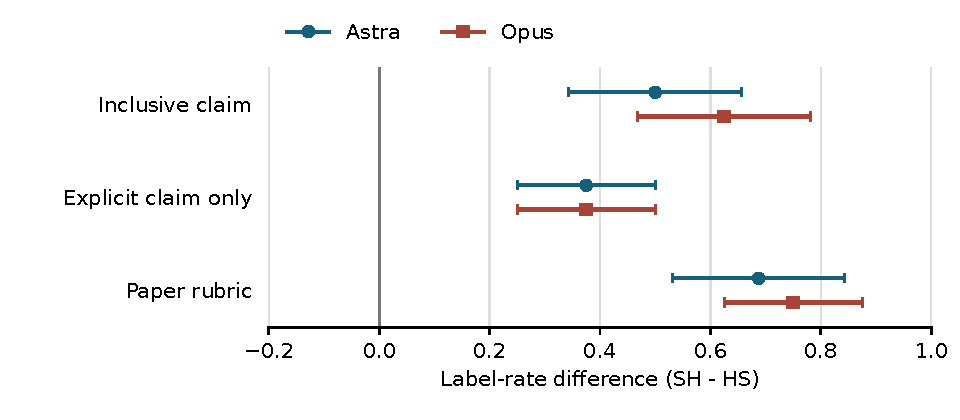
\includegraphics[width=\linewidth]{../evidence/kolibri_presentation/measurement.pdf}
\caption{\textbf{Kolibri's estimated instruction advantage depends on the
scoring rule.} As in Figure~\ref{fig:qwen-extension}, SH--HS compares a
self-referential instruction with a history continuation against the
reverse pairing. GPT-6 Astra and Claude Opus 5.5 score the same
\KEXMainAstraInclusiveSHHSPlannedBlocks{} paired blocks under three rules.
Bars show pointwise 95\% descriptive paired-block bootstrap intervals,
using 10,000 resamples within wording families. These are not the primary
confirmatory intervals: the text retains the simultaneous bounds for the
two planned comparisons. Figure~\ref{fig:kolibri-uncertainty} also shows the
neutral-instruction contrast and the conservative pointwise bounds.}
\label{fig:kolibri-extension}
\end{figure}

The scoring rule again changes the apparent size of the instruction
advantage (Figure~\ref{fig:kolibri-extension}). Opus's inclusive estimate
was \KEXMainOpusInclusiveSHHSCompleteEstimate{}; the two paper-rubric
estimates were \KEXMainAstraPaperSHHSCompleteEstimate{} and
\KEXMainOpusPaperSHHSCompleteEstimate{}. Counting only explicit claims
gave \KEXMainAstraExplicitSHHSCompleteEstimate{} under either reader.
This adds a model with a different architecture and serving precision,
not a controlled test of what those differences cause.
